\chapter{Evaluation}
\label{c:evaluation}

We integrated our columnar storage and techniques into the in-memory GraphflowDB GDBMS. The version of the system we modified stored the edge and vertex properties in a row-oriented fashion as a sequence of variable-sized records indexed by their IDs and partitions the edges by labels and stores them as 8-byte vertex and edge IDs inside CSR. The goal of our experiments is two-fold. First, we show that using columnar storage and compression techniques reduces the memory consumption of the system significantly, by 3.5x, when storing a graph dataset generated by the popular LDBC social network benchmark. Second, we evaluate the query performance benefits and tradeoffs that these techniques provide. In particular, we organize our experiments as follows:
%  We show that redesigning the storage layer of \gls{gdbms} using columns that can harness the structure that exist in data  the graph can compact the storage by up to 3.5x.

\begin{enumerate}
	\item \textbf{Compression in Adjacency Lists:}  In Section~\ref{exp:adjacency-list-exp} we show the reduction in the size of our adjacency lists when applying the storage optimizations from Sections~\ref{c:columnar-storage} and~\ref{columnar-compression}. For each optimization, we state the cause of the reduction in size and query performance effect of the optimization.
		
	\item \textbf{Single-directional Property Pages:} In Section~\ref{exp:property-pages}, we compare the performance of storing edge properties in single-directional property pages, as compared to strictly-ordered single-directional property lists and unordered edge columns.
	
	\item \textbf{Vertex Columns for Single Cardinality Edges vs. CSR Adjacency Lists:}  In Section~\ref{exp:single-cardinality}, we show the effectiveness of storing single cardinality edges in vertex  columns as compared to in CSR format. 
	
	\item \textbf{Prefix Sum-based Null Compression:}  In Section~\ref{exp:prefixSum}, we evaluate the size  and performance tradeoff of compressing our columns with our prefix sum-based null compression scheme. We also compare our technique with the vanilla null compression technique mentioned in~\cite{abadi-sparse-col}.% to show the benefit of using a map instead of iterating over bit-strings.

	\item \textbf{List-based Processing vs Volcano-styled Query Execution:} In Section~\ref{exp:list-based}, we show the performance benefits of list-based processing over Volcano-styled processing.
	
\end{enumerate}

Noticeably missing in our evaluations is comparisons against the other \gls{gdbms} systems and conventional column stores, which we plan to perform as part of future work.

\section{Experimental Setup}

\noindent \textbf{Hardware Setup:} For all our experiments, we use a single machine that has two Intel E5-2670 @2.6GHz CPUs and 512 GB of RAM. The machine has 16 physical cores and 32 logical cores. We only use one logical core. We set the maximum size of the JVM heap to 500 GB and keep JVM's default minimum size.

\begin{figure}
	\centering
	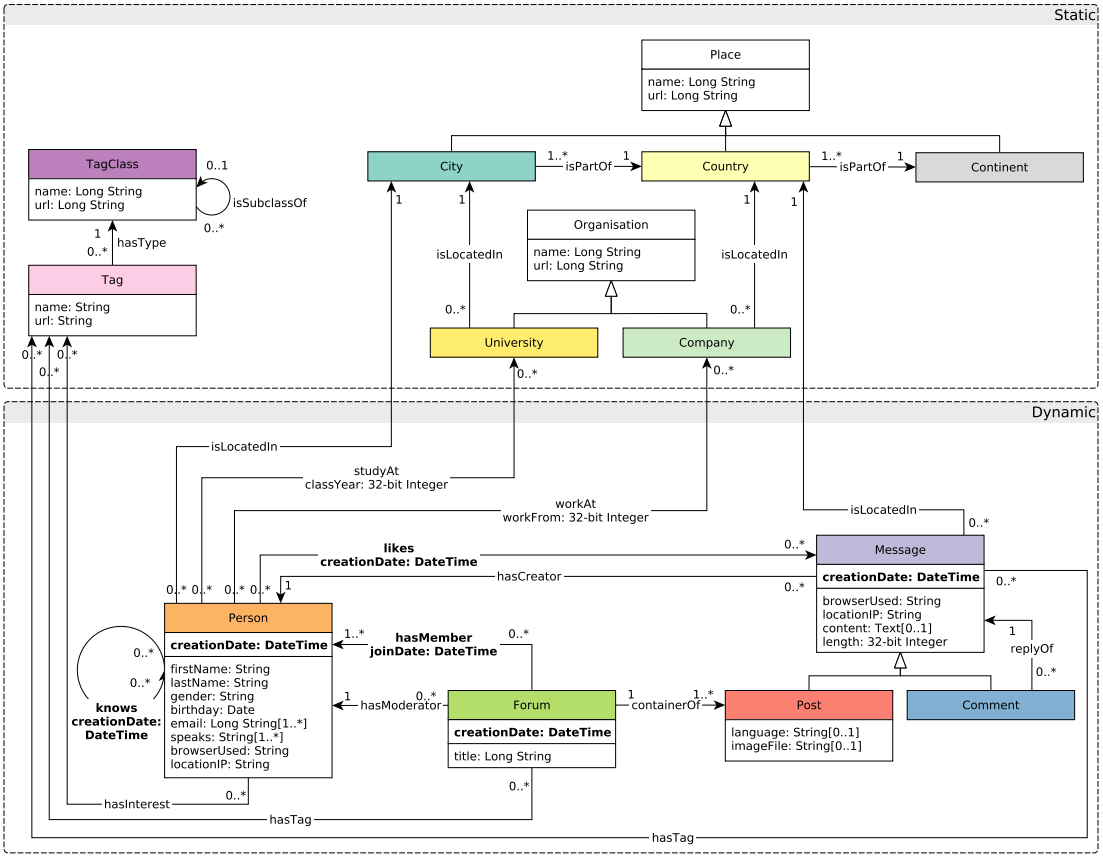
\includegraphics[scale=0.42]{img/ldbc-schema}
	\captionsetup{justification=centering}
	\caption{\gls{ldbc} Graph schema. (Obtained from LDBC SNB specification document v0.3.2)}
	\label{fig:ldbc-schema}
\end{figure}

\noindent \textbf{Dataset:} We use the \gls{ldbc}~\cite{ldbc} dataset generator to generate synthetic graph datasets on which we evaluate all our experiments. \gls{ldbc} is a popular benchmark to generate large social graph data with attributes on nodes and edges. The generated social graph is highly structured which can be seen from the schema in Figure~\ref{fig:ldbc-schema}. In fact all of the edges and edge and vertex properties are structured according to our definition from Chapter~\ref{c:guidelines} but several properties and edges are very sparse. For example, property X on vertices with type X appears in less than X\% of the nodes with type X.\todo{Complete the X's.}  We generate the data at the scale factor of 100 (LDBC100) that consists of over 1.7 billion edges and 0.3 billion vertices. We refer to this dataset as LDBC100

\noindent \textbf{Query Workload:} We use a micro benchmark we generate that consists of 1-, 2-, and 3-hop path queries that optionally contain predicates on vertex and edge properties and aggregations. These queries serve as a stress test for evaluating access to the underlying storage, which our techniques optimize. 
%For instance, a simple 1-hop query tests more rigorously for access from adjacency lists than a query that involves filtering and aggregations. 

\section{Compression in Adjacency Lists}
\label{exp:adjacency-list-exp}

%We introduced several optimizations that can make use of the graph data's structure to drastically compact the representation of edges and vertices in the adjacency lists. 
In this experiment, we demonstrate the memory reduction we get from the columnar storage and compression techniques we described in this thesis that reduce the cost of storing (edgeID, neighborID) pairs in adjacency lists.% that exploits structure in graph data on LDBC100.  
% optimizations on LDBC100 by recording the memory utilization of the adjacency lists across different %configurations which we describe momentarily.
We create multiple configurations on GraphflowDB, each with a different set of optimizations. Below are the descriptions of the configurations we evaluate the memory usage on. Each configuration builds on top of previous in the list. 

\begin{enumerate}
	\item \texttt{GF-OLD:} This is our baseline configuration that represents edges and vertices in the adjacency list as 8-byte identifiers. All the edges are stored in the 2-level CSR structure and are not compressed.
	\item \texttt{+COLS}: Uses vertex columns from single cardinality edge labels. 
	\item \texttt{+NEW-IDS}: Introduces our new vertex and edge identification schemes.
	\item \texttt{+0-SUPR}: Implements leading 0 suppression in the components of vertex and edge IDs in adjacency lists.
	\item \texttt{+OMIT}: Omits neighbor vertex label and positional offsets of edge IDs when they can be inferred from the structure.
	\item \texttt{+NULL}: Implements prefix sum-based null compression on adjacency lists (or vertex columns for single cardinality edges).
\end{enumerate}

\begin{table}
	\centering
	\bgroup
	\setlength{\tabcolsep}{8pt}
	\def\arraystretch{1.2}%  1 is the default, change whatever you need
	\begin{tabular}{ |c|c|c|c|c|c|c| } 
		\hline
		& \texttt{GF-OLD} & \texttt{+COLS} & \texttt{+NEW-IDS} & \texttt{+0-CMPRS} & \texttt{+OMIT}& \texttt{+NULL} \\ 
		\hline \hline
		\multirow{2}{120pt}{Fwd. Adjacency Lists}& 38.25 & 33.25 & 27.22 & 16.35 & 11.14 & 10.53 \\ 
		& & \textbf{+1.15x} & \textbf{+1.22x} & \textbf{+1.66x} & \textbf{+1.47x} & \textbf{+1.06x} \\ 
		\hline
		\multirow{2}{120pt}{Bwd. Adjacency Lists}& 37.93 & 37.50 & 30.93 & 18.75 & 12.79 & 11.15 \\ 
		& & \textbf{+1.01x} & \textbf{+1.21x} & \textbf{+1.65x} & \textbf{+1.47x} & \textbf{+1.15x} \\ 
		\hline
		\multirow{3}{120pt}{Total (GB)\\Bytes Per Edge\\} & 76.18 & 70.75 & 58.15 & 35.10 & 23.93 & 21.68 \\ 
		 & 23.04 & 21.39 & 17.58 & 10.61 & 7.24 & 6.50 \\ 
                 & & \textbf{1.08x} & \textbf{1.31x} & \textbf{2.17x} & \textbf{3.18x} & \textbf{3.55x} \\  
%		\hline \hline
%		\multirow{3}{80pt}{Bytes per edge}& 23.04 & 21.39 & 17.58 & 10.61 & 7.24 & 6.50 \\ 
%		& & \textbf{1.08x} & \textbf{1.31x} & \textbf{2.17x} & \textbf{3.18x} & \textbf{3.55x} \\ 
		\hline
	\end{tabular}
	\egroup
	\captionsetup{justification=centering}
	\caption{Memory utilization (in GB) by Adjacency lists of  LDBC100 when adding our optimizations one at a time. Each column $i$ indicates an optimization $i$ and in the rows for forward and backward lists indicate the additional reduction factor of applying optimization $i$ on top of the previous optimizations to the left of $i$. In contrast, in the row on total memory consumption/bytes per edge, each column $i$ indicates the cumulative reduction factor (compared to \texttt{GF-OLD}) of applying all optimizations from left until $i$.}
	\label{tbl:mem1}
\end{table}

\begin{figure}
	\centering
	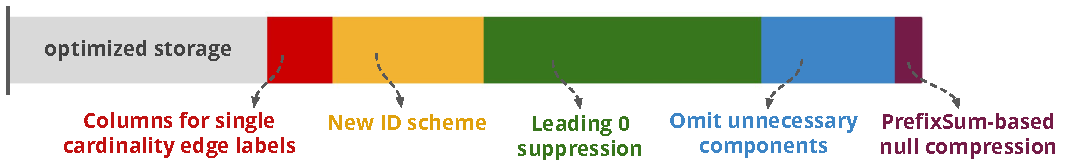
\includegraphics[scale=0.75]{img/opti-breakup}
	\captionsetup{justification=centering}
	\caption{Breakup of memory gains by applying different optimizations on Adjacency Lists of \gls{ldbc} scale factor 100 dataset.}
	\label{fig:opti-breakup}
\end{figure}

Table~\ref{tbl:mem1} shows how much memory (in GB) the adjacency lists take when storing the edges of LDBC100 across different configurations.  Figure~\ref{fig:opti-breakup} gives the breakup of memory gain per optimization. Memory gain in \texttt{+COLS} is attributed to the fact that 8 out of 15 edge labels are single cardinality and stored in vertex columns in at least one direction. \texttt{+NEW-IDS} gains ({\raise.17ex\hbox{$\scriptstyle\sim$}}4 bytes per edge) by storing edges in smaller than 8 bytes, while \texttt{+OMIT} gains ({\raise.17ex\hbox{$\scriptstyle\sim$}}3 bytes per edge) from not storing edge's positional offsets and neighbour's vertex label for 10 out of 15 edge labels. We see modest benefits in \texttt{+NULL} ({\raise.17ex\hbox{$\scriptstyle\sim$}}0.75 bytes per edge) since empty adjacency lists are infrequent in LDBC100.

All of these optimizations also improve query performance, with the exception of \texttt{+NULL}, which incurs a modest query slow down. We will evaluate the performance gains and tradeoffs of \texttt{+COLS} and \texttt{+NULL} are evaluated in Sections~\ref{exp:single-cardinality} and ~\ref{exp:prefixSum} respectively. 
We will not evaluate the benefits of leading 0 suppression but we note that this also improves performance because we do not have to decode a particular value and hence, and have modest gains because we copy less data into tuples from the adjacency lists.

%Further, the memory utilization of \gls{ldbc} 300 (5.27B edges, 0.6B vertices) with our set of optimizations was 63.45GB. In all, we are able to scale the new GraphflowDB (with our new storage layer) to store up to 10.5B edges, along with vertex and edge properties, of \gls{ldbc} data on a single machine with 500GB of main memory. This is {\raise.17ex\hbox{$\scriptstyle\sim$}}15x increase in scalability compared to old GraphflowDB with unoptimized storage.

\section{Effectiveness of Single-Directional Property Pages}
\label{exp:property-pages}

In this experiment, we show the benefits of keeping the edge properties grouped in single-directional property pages compared to using edge columns that store the edge properties in an unordered way. 
Recall that one alternative design we described was using  single-directional property lists to store edge properties. This design had the advantage that edge properties would be kept in exactly the same order as they appear in adjacency lists, but it can make updates significantly slower, specifically for systems that keep edges in sorted order. However, this design may still be a viable design for some GDBMSs and as a point of reference we also evaluate its benefits. 
%We also demonstrate that keeping edge properties in property pages instead of single-directional property lists is a reasonable trade-off as we lose modest performance. but significantly win over edge columns. 
To test the performance benefits of single-directional property pages and lists, we configure GraphflowDB  in 3 different ways (all using our new ID schemes):

\begin{enumerate}
	\item \texttt{EDGE COLS:} Stores edge properties in edge column in the order they were inserted into the database, so properties of edges in a particular adjacency list (forward or backward) can appear anywhere in this column. We ensure that the insertion order is random. % in  If there are $|E|$ many e For example, the edge properties of label \texttt{knows} are stored in columns that are oblivious to the location of \texttt{knows} edges in either the forward or backward adjacency lists. 
	\item \texttt{PROP LISTS:} Edge properties are stored in the single-directional property lists. We pick the forward list for $n-n$ multiplicity edges. Therefore these property lists mimic the forward adjacency lists and gives sequential reads when edge properties of a forward adjacency list are read.
	
	\item \texttt{PROP PAGES:} Edge properties are stored in pages by combining $n=128$ property lists of the previous solution and appear in insertion order. This solution provides close-by reads when edge properties of a forward adjacency list are read.
\end{enumerate}

\begin{table}
	\centering
	\bgroup
	\setlength{\tabcolsep}{8pt}
	\def\arraystretch{1.2}%  1 is the default, change whatever you need
	\begin{tabular}{ |c|c|c|c| } 
		\hline
		& \textbf{1-hop} & \textbf{2-hop} & \textbf{3-hop} \\
		\hline \hline
		\texttt{EDGE COLS}& 3.42 & 308.18 & 966.04\\ 
		\hline 
		\multirow{2}{*}{\texttt{PROP PAGES}} & 1.22 & 152.89 & 512.24 \\ 
		& \textbf{2.80x} & \textbf{2.03x} & \textbf{1.87} \\ 
		\hline
		\multirow{2}{*}{\texttt{PROP LISTS}}& 1.03 & 125.65 & 372.44 \\ 
		& \textbf{3.32x} & \textbf{2.42x} & \textbf{2.59}\\ 
%		\hline \hline
%		\texttt{PROP PAGES} vs \texttt{PROP LISTS} & 1.19x & 1.22x & 1.37x \\
		\hline
	\end{tabular}
	\egroup
	\captionsetup{justification=centering}
	\caption{Runtime (in sec) of k-hop queries for different configurations of edge property storage on LDBC100.}
	\label{tbl:mem2}
\end{table}

As our workload, we use 1- 2- and 3-hop queries that use the \texttt{knows} edge label of the \gls{ldbc} schema (Figure~\ref{fig:ldbc-schema}) that compare each query edge's \texttt{creationDate} property to be greater than the previous edge's. 1-hop and 2-hop queries run for all vertices of \texttt{person} while we run 3-hop for only 25000 vertices to make the queries faster. For each query, we only consider the plan that matches vertices from left to right in the forward direction. This way, we are ensure cache locality for \texttt{PROP-LISTS} and \texttt{PROP-PAGES}. Table~\ref{tbl:mem2} shows the performance of queries on 3 configurations. We observe that the queries benefit significantly from localizing edge properties in the storage. Compared to \texttt{EDGE COLS}, we see up to 2.8x improvement for \texttt{PROP PAGES} and up to 3.32x improvements for \texttt{PROP LISTS}. Recall also that using \texttt{PROP PAGES} or \texttt{PROP LISTS} also reduces our storage because the amount of bytes required to identify edges within a list or a property page is smaller than the bytes needed to identify an edge within an entire edge column. In a system that uses fixed size IDs, which in-memory systems optimized for performance should do, 8 bytes is needed to identify edges in billion-scale graphs while 4 bytes is sufficient to identify edges within a list or property page. Finally, note that the benefits we get from \texttt{PROP PAGES} will depend on $n$, in particular as $n$ approaches 1, \texttt{PROP PAGES} design reduces to \texttt{PROP LISTS}. We have not performed this experiment but as $n$ gets smaller we expect the performance differences between \texttt{PROP LISTS} and \texttt{PROP PAGES} to reduce.

% In addition, using property lists or pages allows us to use positional offsets that need to identify edges within a list of a property page (so 128 lists). 
%The benefits decrease with the size of query because the last operators in a query plan flush the pages from which earlier operators read. However, both property lists and pages still guarantee benefits over unordered \texttt{EDGE COLS}. On the other hand, storing the edge properties in the update-friendly property pages only slightly degrades the performance of queries (1.19-1.37x). This depends on the value of $n$, i.e, the number of property lists that we put together on a page. The average number of \texttt{knows} edges per \texttt{person} vertex is {\raise.17ex\hbox{$\scriptstyle\sim$}}44 edges while $n=128$. A lower $n$ means that properties of edges in an adjacency lists appear closer in the page and hence, provide more localized reads.

\section{Vertex Columns for Single Cardinality Edges vs CSR Adjacency Lists}
\label{exp:single-cardinality}

Storing single cardinality edges in vertex columns ensure two benefits: (i) direct access into the edge without indirection into CSR, and 2) does not need to store offsets of the CSR. We showed the memory gains of storing edges in vertex columns in Section~\ref{exp:adjacency-list-exp}. We next compare the performance benefits of using vertex column vs adjacency lists in CSR format under two settings: (i) when empty lists (or edges because of single cardinality) are not null compressed; and (ii) when they are null compressed. We create 4 configurations of GraphflowDB to run our queries on:

\begin{enumerate}
	\item \texttt{V-COL-UNC:} Single cardinality edge label edges are stored in vertex columns and are not compressed. 
	\item \texttt{CSR-UNC:} Single cardinality edge label edges are stored in CSR format and are not compressed.
	\item \texttt{V-COL-C:} Null compressed version of \texttt{V-COL-UNC}. This is equivalent to \texttt{+NULL} configuration in Section~\ref{exp:adjacency-list-exp}.
	\item \texttt{CSR-C:} Null compressed version of \texttt{CSR-UNC}.
\end{enumerate}

The workload consists of simple 1-, 2-, and 3-hop queries on the \texttt{replyOf} edge between \texttt{comment} vertices in the \gls{ldbc} schema. The \texttt{replyOf} edge label has \texttt{n-1} cardinality, hence, we keep the forward edges as a special property of \texttt{comment} vertex label. Moreover, our workload queries do not do any predicate evaluation and the final output of the query is an aggregated count. This assures that \texttt{JOIN} operation in the query plan is the only dominant operation. Again, for each query, we evaluate only on the plan that matches the vertices sequentially and joins in the forward direction.

\begin{table}
	\centering
	\begin{subtable}{1\textwidth}
		\centering
		\bgroup
		\setlength{\tabcolsep}{8pt}
		\def\arraystretch{1.2}%  1 is the default, change whatever you need
		\begin{tabular}{ |c|c|c|c|c| }
			\hline
			& \textbf{1-hop} & \textbf{2-hop} & \textbf{3-hop} & \textbf{Memory (in MB)} \\ 
			\hline \hline
			\texttt{CSR-UNC}& 7.03 & 9.13 & 9.60 & 1266.56 \\ 
			\hline
			\multirow{2}{*}{\texttt{V-COL-UNC}}& 4.34 & 5.80 & 5.85 & 839.93 \\ 
			& \textbf{1.62x} & \textbf{1.57x} & \textbf{1.64x} & \textbf{1.51x} \\ 
			\hline
		\end{tabular}
		\egroup
		\captionsetup{justification=centering}
		\caption{Uncompressed}
		\label{tbl:s1}
	\end{subtable}
	\begin{subtable}{1\textwidth}
		\centering
		\bgroup
		\setlength{\tabcolsep}{8pt}
		\def\arraystretch{1.2}
		\begin{tabular}{ |c|c|c|c|c| } 
			\hline
			& \textbf{1-hop} & \textbf{2-hop} & \textbf{3-hop} & \textbf{Memory (in MB)} \\ 
			\hline \hline
			\texttt{CSR-C}& 7.78 & 10.40 & 11.23 & 905.23 \\ 
			\hline
			\multirow{2}{*}{\texttt{V-COL-C}}& 5.23 & 8.28 & 8.41 & 478.86 \\ 
			& \textbf{1.49x} & \textbf{1.26x} & \textbf{1.34x} & \textbf{1.89x} \\ 
			\hline
		\end{tabular}
		\egroup
		\captionsetup{justification=centering}
		\caption{Null Compressed}
		\label{tbl:s2}
	\end{subtable}
	\captionsetup{justification=centering}
	\caption{Vertex property columns vs. 2-level CSR adjacency lists for storing single cardinality edges: Query runtime (in sec) and Memory usage (in MB)  }
\end{table}

Tables~\ref{tbl:s1} and ~\ref{tbl:s2} shows the result of queries on uncompressed and null compressed configurations respectively. We observe up to 1.62x performance gains between uncompressed variants of vertex columns and CSR (i.e., \texttt{V-COL-UNC} vs \texttt{CSR-UNC}) and up to 1.49x gains between null compressed variants (i.e.,  \texttt{V-COL-C} vs \texttt{CSR-C}). The last column of the tables report the size of the adjacency lists or vertex column storing \texttt{replyOf} edges. Here, vertex column uses half as much space as adjacency lists, when the data is kept compressed. In LDBC100, out of {\raise.17ex\hbox{$\scriptstyle\sim$}}220M \texttt{comment} vertices 50.5\% have empty forward adjacency list, i.e, do not have an outward \texttt{replyOf} edge. This is reflected in vertex columns between \texttt{V-COL-UNC} and \texttt{V-COL-C}, as the memory reduces by 1.75x (839.93MB vs 478.86MB), unlike their CSR counterparts that stores offsets as extra and thus, compression reduces memory by only 1.4x (1266.56 vs 905.23). These results verify that using vertex columns for single-cardinality edges not only saves space, but also improves query performance (irrespective of whether or not the edges/lists are null compressed or not).

\section{Effectiveness of Prefix Sum-based Null Compression}
\label{exp:prefixSum}

We demonstrate the memory performance tradeoff of prefix sum-based null compression when compressing both sparse property columns as well as empty adjacency lists. We evaluate two aspects of our technique: (i) storage and random access efficacy against uncompressed and vanilla null compressed columns; and (ii) query performance on compressed and uncompressed vertex columns and adjacency lists.

%\subsection{Stress Test} 

\begin{figure}
	\hspace*{-25pt}
	\begin{subfigure}{0.55\textwidth}
		\centering
		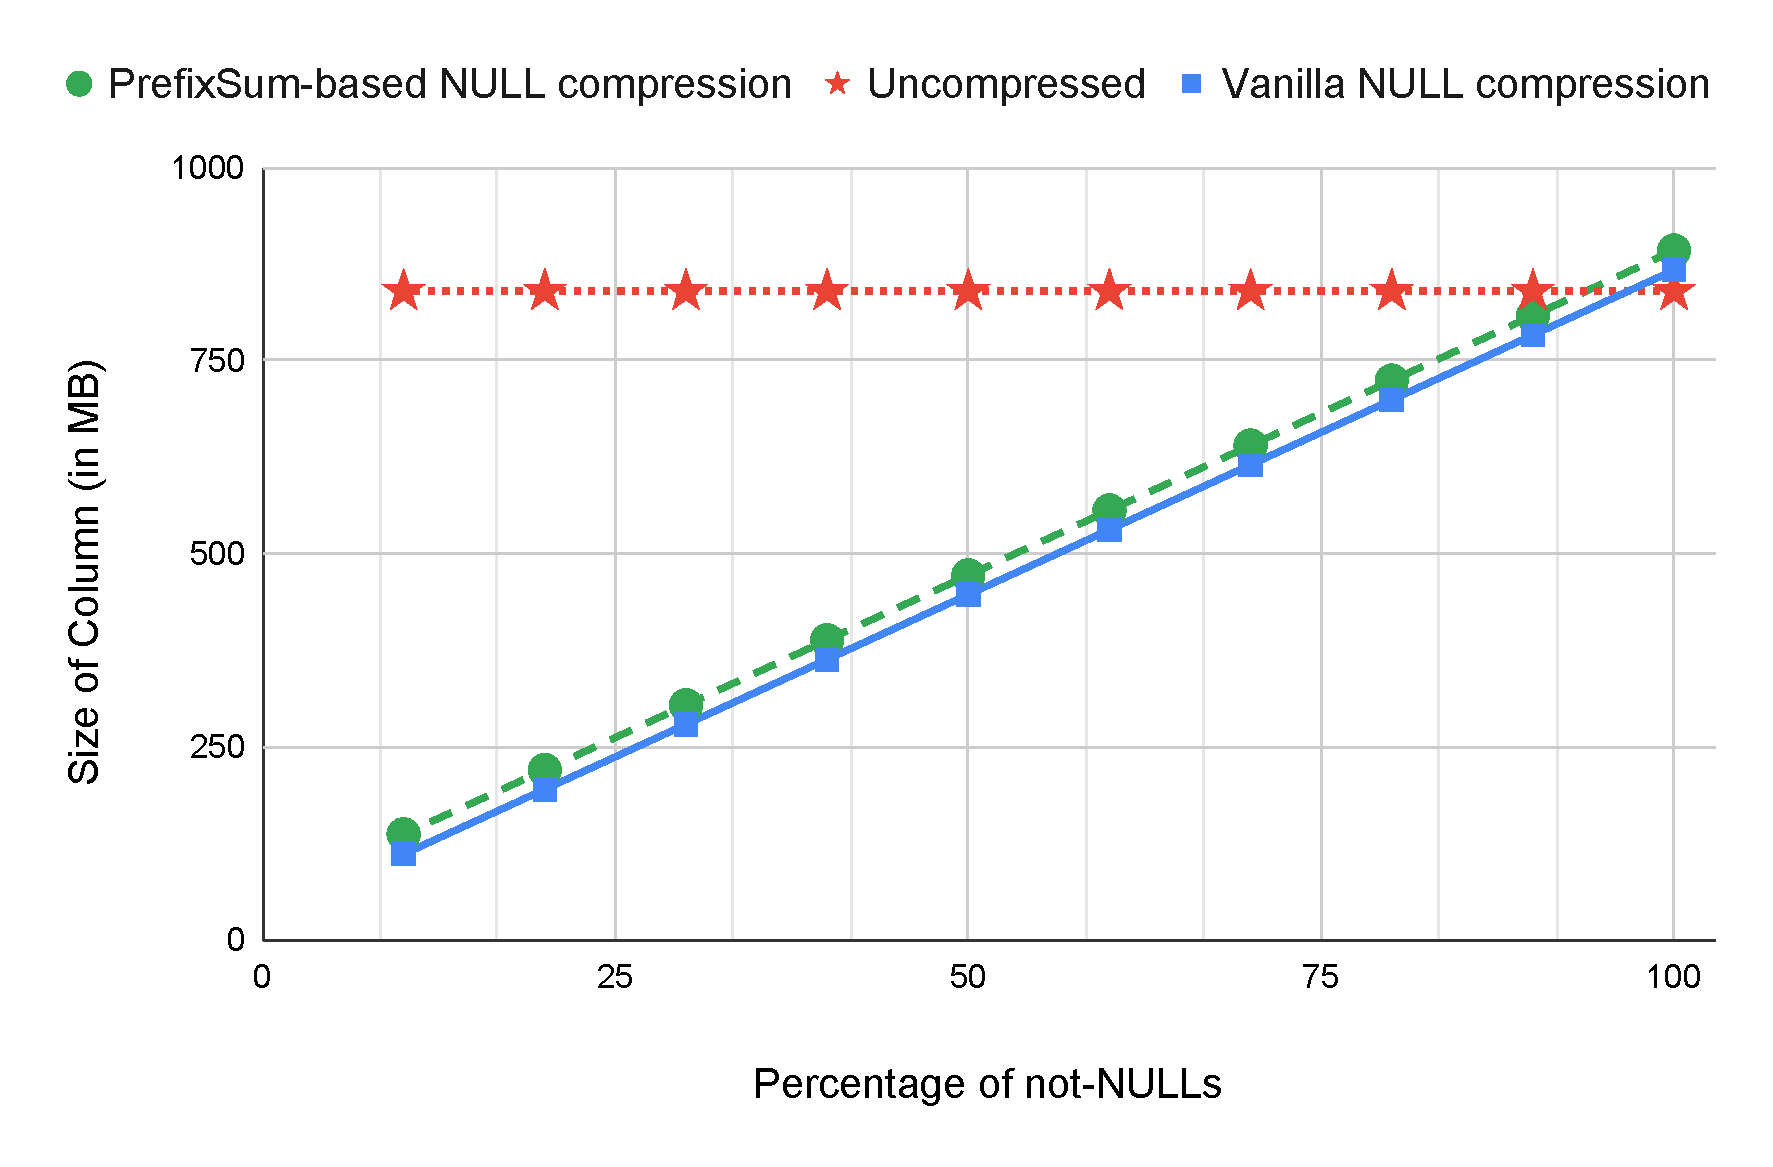
\includegraphics[scale=0.30]{img/pref-space}
		\captionsetup{justification=centering}
		\caption{Memory usage}
		\label{fig:pref-space}
	\end{subfigure}
	\begin{subfigure}{0.55\textwidth}
		\centering
		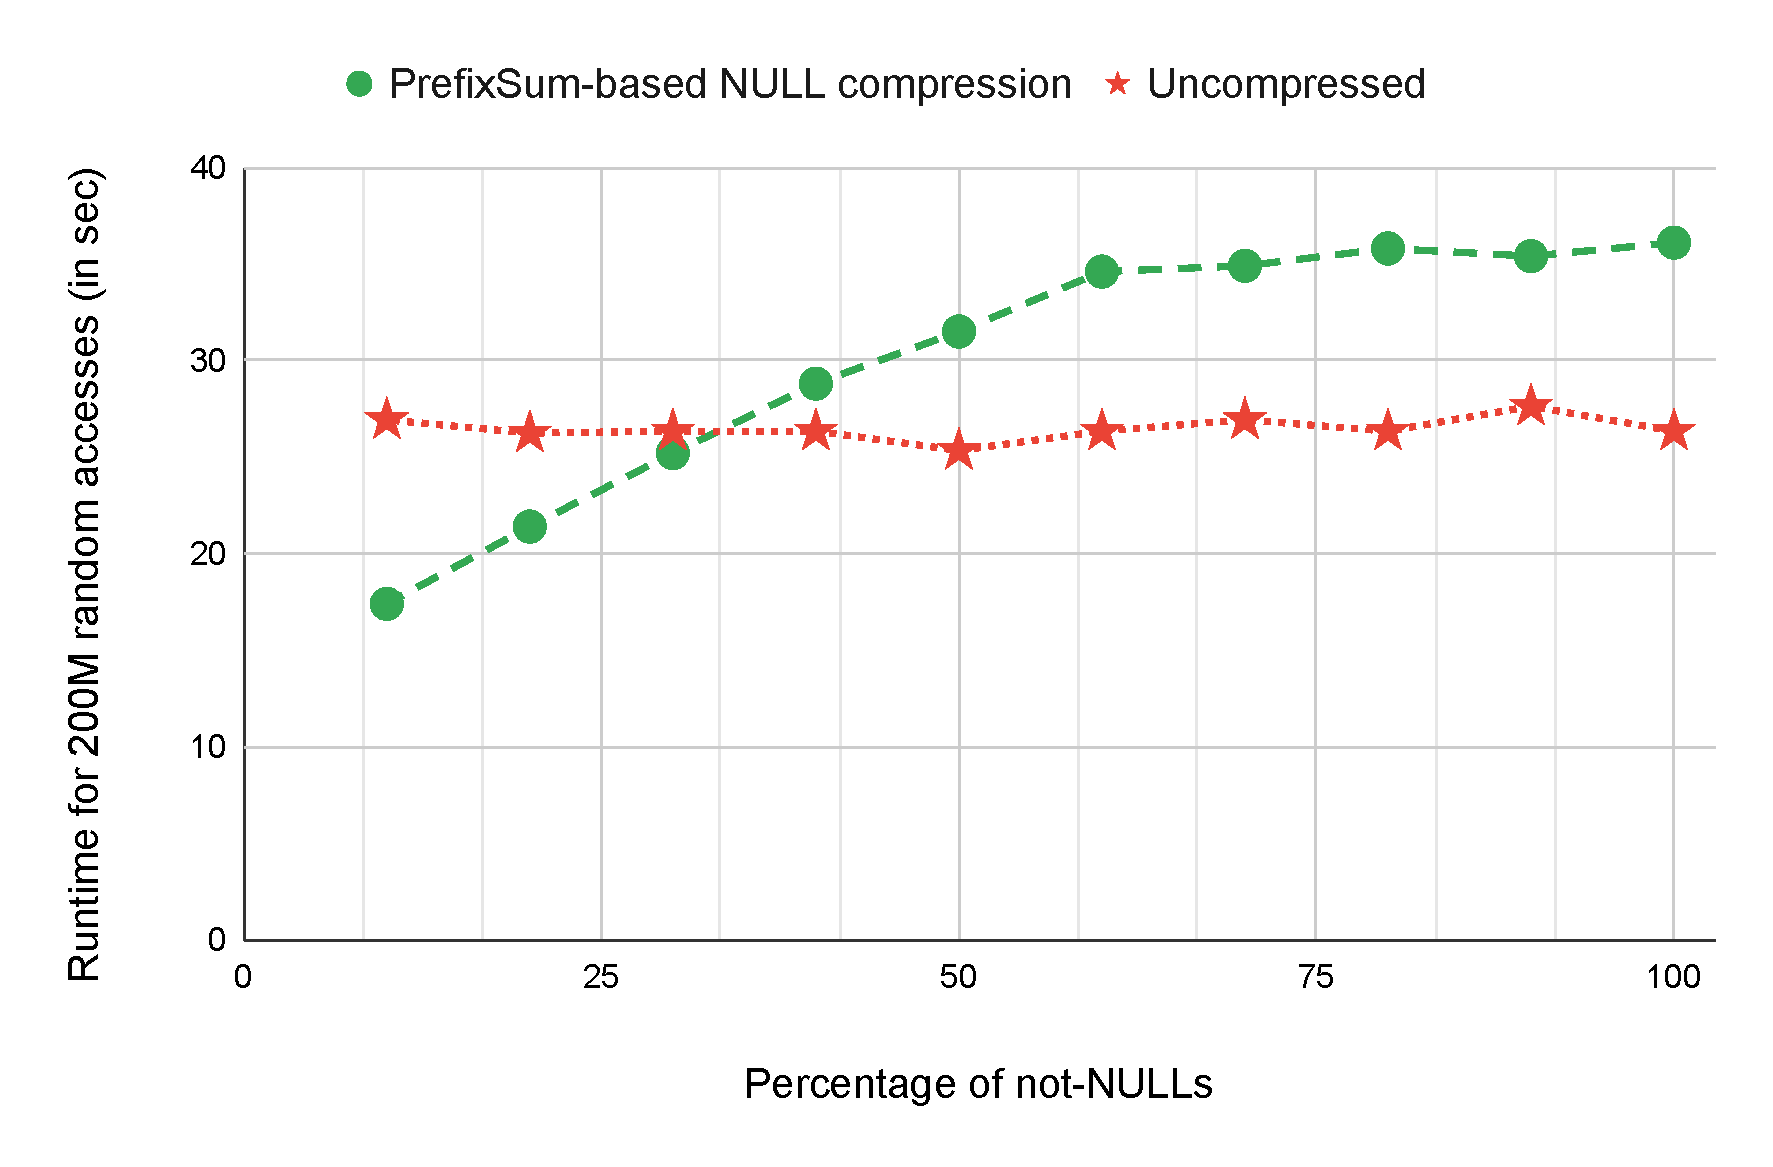
\includegraphics[scale=0.30]{img/pref-perf}
		\captionsetup{justification=centering}
		\caption{Performance on random accesses}
		\label{fig:pref-perf}
	\end{subfigure}
	\captionsetup{justification=centering}
	\caption{Memory and performance on random accesses for Uncompressed, prefix sum-based NULL compressed and vanilla NULL compressed columns.}
	\label{fig:pref-stress}
\end{figure}

The goal of our first experiment is to compare uncompressed, prefix sum-based null compressed and vanilla null compressed (as implemented in ~\cite{abadi-sparse-col}) columnar data-structure for memory usage and performance on random reads. We design a micro-benchmark to stress test the access performance when performing random accesses to a null compressed column. We use the \texttt{creationDate} property of 220M \texttt{comment} vertices in LDBC100 and create multiple versions of it, each with different percentage of non-null values. On each version, we do the necessary compression and measure the time taken to do 200M access to random locations in the column. 

Figures~\ref{fig:pref-space} and~\ref{fig:pref-perf} show memory usage and performance on 200M random read queries respectively, for uncompressed, prefix sum-based null compressed and vanilla null compressed column of \texttt{creationDate} property of \texttt{comment} vertex label. We omit the performance number of vanilla null compression as they were significantly higher than the other two configurations ($>$20x). Our prefix sum-based  compression technique requires slightly more memory than vanilla null compression technique (2-bit for each element vs. 1-bit overhead in vanilla compression). However, introducing prefix sums and map lookups in stead of iterations over bit-strings of each block provide significant performance benefits. We observe at most 1.38x slow down the performance compared to the uncompressed column, which has no decompression cost. Surprisingly, accesses in prefix-sum based compression can even be faster than accesses to an uncompressed column when the column is very sparse ($<30\%$ non-null values). This is because testing for null at a location is a constant time operation and when most of the accesses return null, in a null compressed column, the iterators return a single global variable that keeps  the null value for the data type. Instead, in an uncompressed column, the null value from the column is copied, which has a higher chance of a CPU cache miss. 

%\subsection{Query Performance}

Tables~\ref{tbl:s1} and~\ref{tbl:s2} already compares reading edges from compressed and uncompressed adjacency lists and vertex columns. Reading edges from CSR adjacency lists and vertex columns that are null compressed by our technique are on average 1.14x and 1.3x slower than their uncompressed variant respectively. However, for 50\% null values, they gain 50\% and 25\% in storage respectively. 

\begin{table}
	\centering
	\bgroup
	\setlength{\tabcolsep}{8pt}
	\def\arraystretch{1.2}%  1 is the default, change whatever you need
	\begin{tabular}{ |c|c|c|c| } 
		\hline
		& \textbf{1-hop} & \textbf{2-hop} & \textbf{3-hop} \\
		\hline \hline
		\texttt{V-COL-UNC}& 12.78 & 14.47 & 14.95\\ 
		\hline
		\multirow{2}{*}{\texttt{V-COL-C}}& 14.65 & 16.00 & 16.98 \\ 
		& \textbf{1.15x} & \textbf{1.11x} & \textbf{1.14x}\\ 
		\hline  
	\end{tabular}
	\egroup
	\captionsetup{justification=centering}
	\caption{Runtime (in sec) of k-hop queries on compressed and uncompressed vertex column on LDBC100.}
	\label{tbl:s3}
\end{table}

In our second experiment, we evaluate accessing vertex properties from compressed and uncompressed vertex columns using k-hop queries. We use the \texttt{V-COL-C} and \texttt{V-COL-UNC} configurations and keep the edge storage uncompressed. We run the workload from Section~\ref{exp:single-cardinality} consisting of k-hop queries over \texttt{replyOf} edges. These queries are extended to include a condition that a \texttt{comment} $b$ is made on another \texttt{comment} $a$ such that $b$ has a \texttt{creationDate} that is within $\delta$ timespan of $a$'s. Table~\ref{tbl:s3} shows our results. Using compressed storage slows down our queries by at most 1.14x. Therefore compared to the vanilla null compression schemes, which are not practical, our prefix sum-based null compression scheme is a practical compression scheme that offers a good performance and memory trade-off.

\section{List-based Processing vs. Volcano-styled Query Execution}
\label{exp:list-based}

We next provide a preliminary set of experiments that compare the performance of our list-based processing to Volcano-style processing. We use the GraphflowDB with our new columnar storage under two configurations; (i) \texttt{VOLCANO}, that uses the conventional Volcano-styled processor, which we achieve by ensuring plans do not use our vector-oriented operators (e.g., \texttt{LIST-JOIN}); and (ii) \texttt{LIST-BASED} that uses our new list-based operators. Our workload consist of simple 1-, 2-, and 3-hop queries that read the \texttt{replyOf} edges of the \texttt{person} vertex in LDBC100 and returns the count of final matches. We evaluate the queries on similar plans that perform the same sequence of joins.
Table~\ref{tbl:list-volcano} shows the query performance of the 2 query processors. As we expect, list-based processor is more performant than Volcano-style processor. Specifically, we obtain between 1.33x and 2.72x runtime speed up. Our evaluation of list-based processing is currently very preliminary and at the time of this writing we are in the process of implementing and optimizing our list-based operators. We leave a more extensive evaluation of the benefits and limitations of list-based processing to future work.

%However, when the query reads the property of last vertex (see Table~\ref{tbl:s5}), the performance drops significantly and we see the maximum speed-up of only 1.13x. The reason for this difference is the fact that while reading properties, the \texttt{LIST PROPERTY READER} has to iterate over the contents of the adjacency list being joined by the \texttt{LIST JOIN}, which in our current implementation is a costly operation. However, iteration over the list can be completely bypassed in case other operators in the query plan do not depend on the values of the list and hence, saves computation. 
% on both query processors, except that the last \texttt{JOIN} operation and \texttt{PROPERTY READER} (that depends on the last \texttt{JOIN}) operates on the list in case of list-based query processor.

\begin{table}
	\centering
%	\begin{subtable}{1\textwidth}
		\centering
		\bgroup
		\setlength{\tabcolsep}{8pt}
		\def\arraystretch{1.2}%  1 is the default, change whatever you need
		\begin{tabular}{ |c|c|c|c| }
			\hline
			& \textbf{1-hop} & \textbf{2-hop} & \textbf{3-hop} \\ 
			\hline \hline
			\texttt{VOLCANO}& 3.12 & 259.34 & 734.72 \\ 
			\hline
			\multirow{2}{*}{\texttt{LIST-BASED}}& 2.35 & 95.24 & 313.67 \\ 
			& \textbf{1.33x} & \textbf{2.72x} & \textbf{2.34x} \\ 
			\hline
		\end{tabular}
		\egroup
		\captionsetup{justification=centering}
		\caption{Without reading vertex property}
%		\label{tbl:s4}
%	\end{subtable}
%	\begin{subtable}{1\textwidth}
%		\centering
%		\bgroup
%		\setlength{\tabcolsep}{8pt}
%		\def\arraystretch{1.2}
%		\begin{tabular}{ |c|c|c|c| }
%			\hline
%			& \textbf{1-hop} & \textbf{2-hop} & \textbf{3-hop} \\ 
%			\hline \hline
%			\texttt{VOLCANO}& 3.35 & 350.54 & 922.35 \\ 
%			\hline
%			\multirow{2}{*}{\texttt{LIST-BASED}}& 3.10 & 310.21 & 810.53 \\ 
%			& \textbf{1.08x} & \textbf{1.13x} & \textbf{1.12x} \\ 
%			\hline
%		\end{tabular}
%		\egroup
%		\captionsetup{justification=centering}
%		\caption{With reading vertex property}
%		\label{tbl:s5}
%	\end{subtable}
	\label{tbl:list-volcano}
	\captionsetup{justification=centering}
	\caption{Runtime (in sec) for two set of k-hop queries using volcano-styled query processing and our new list-based query processing.  }
\end{table}


















